\chapter{Agreement}
\label{ch:agreement}

If the reconstruction score cannot tell a true name from a wrong one, something else must. This chapter
shows that the verbalizer's own samples can: a name it writes every time is usually true, and a name it
writes once is usually not.

\section{Consensus}

Each activation has $K=4$ independently sampled explanations $z_1,\dots,z_K$. For every name $n$ that appears
in any of them, I count how many contain it:
\begin{equation}
c(n) = \sum_{k=1}^{K} \mathbf{1}\bigl[\, n \in N(z_k) \,\bigr].
\label{eq:count}
\end{equation} Figure~\ref{fig:consensus} shows how often a name is true at each
count, pooling distances 1, 4 and 16. Distance~0 is left out of the pooled figure because the true name is
always present there, which would flatter the result.

\begin{figure}[t]
\centering
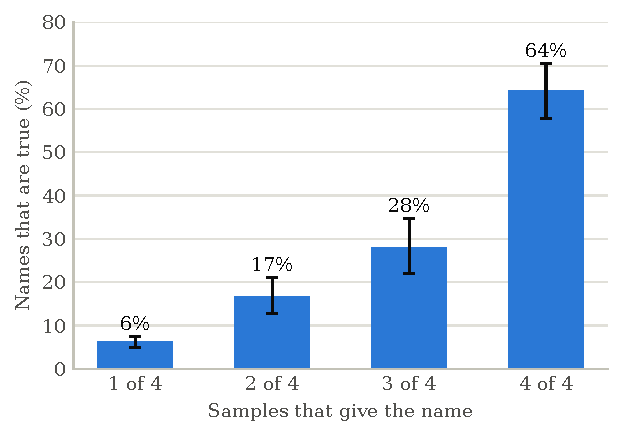
\includegraphics[width=0.6\linewidth]{consensus}
\caption[Names that more samples agree on are more often true]{Names that more samples agree on are more
often true. Natural text, distances 1, 4 and 16 pooled, 3{,}489 names; 95\% intervals.}
\label{fig:consensus}
\end{figure}

A name given by one sample is true 6\% of the time. A name given by all four is true 64\% of the time. As a
score for ranking names, the agreement count has an AUC of 0.80, and it holds up at every distance
(Table~\ref{tab:consensus}).

\begin{table}[t]
\centering
\footnotesize
\setlength{\tabcolsep}{4pt}
\begin{tabular}{@{}lllll@{}}
\toprule
\shortstack[l]{Tokens after\\entity} & 1 of 4 & 2 of 4 & 3 of 4 & 4 of 4 \\
\midrule
0 & 0.0 {\scriptsize[0.0, 0.0]} (717) & 0.0 {\scriptsize[0.0, 0.0]} (148) & 1.3 {\scriptsize[0.0, 3.8]} (78) & 87.5 {\scriptsize[84.8, 90.3]} (616) \\
1 & 5.2 {\scriptsize[3.8, 6.8]} (1{,}113) & 14.2 {\scriptsize[10.1, 18.4]} (240) & 20.3 {\scriptsize[14.1, 27.3]} (182) & 66.4 {\scriptsize[59.7, 73.0]} (348) \\
4 & 7.8 {\scriptsize[5.9, 10.0]} (667) & 20.0 {\scriptsize[11.5, 30.0]} (115) & 39.3 {\scriptsize[28.9, 50.7]} (84) & 62.4 {\scriptsize[53.0, 71.7]} (109) \\
16 & 6.1 {\scriptsize[4.1, 8.5]} (478) & 19.3 {\scriptsize[11.4, 28.4]} (83) & 39.0 {\scriptsize[21.4, 57.9]} (41) & 44.8 {\scriptsize[26.9, 62.1]} (29) \\
1, 4 and 16 & 6.2 {\scriptsize[5.0, 7.5]} (2{,}258) & 16.7 {\scriptsize[12.7, 21.1]} (438) & 28.0 {\scriptsize[22.0, 34.8]} (307) & 64.2 {\scriptsize[57.7, 70.5]} (486) \\
\bottomrule
\end{tabular}

\caption[Precision of a name by how many samples give it]{Precision of a name (\%) by how many of the four
samples give it, with the number of names in brackets. Natural text; 95\% intervals.}
\label{tab:consensus}
\end{table}

\section{Filter}

This suggests a filter that needs no training: keep a name only if $c(n) \ge m$ for some threshold $m$. Table~\ref{tab:filter} shows the trade-off in the terms of retrieval, treating the names as
retrieved items.

\begin{table}[t]
\centering
\small
\begin{tabular}{@{}lllll@{}}
\toprule
\shortstack[l]{Keep a name if\\given by} & \shortstack[l]{Wrong names\\removed} & \shortstack[l]{True names\\kept} & Precision & Names left \\
\midrule
None & 0 & 100 & 17.5 {\scriptsize[15.1, 20.1]} & 3{,}489 \\
At least 2 of 4 & 73.6 {\scriptsize[69.9, 77.3]} & 77.2 {\scriptsize[73.5, 80.6]} & 38.3 {\scriptsize[33.5, 43.4]} & 1{,}231 \\
At least 3 of 4 & 86.3 {\scriptsize[83.9, 88.6]} & 65.2 {\scriptsize[61.6, 68.9]} & 50.2 {\scriptsize[44.6, 56.2]} & 793 \\
All 4 & 94.0 {\scriptsize[92.7, 95.2]} & 51.1 {\scriptsize[46.3, 55.9]} & 64.2 {\scriptsize[57.7, 70.5]} & 486 \\
\bottomrule
\end{tabular}

\caption[The agreement filter as a precision--recall trade-off]{The agreement filter as a
precision--recall trade-off (\%). Natural text, distances 1, 4 and 16 pooled; 95\% intervals. ``True names
kept'' is recall relative to no filter.}
\label{tab:filter}
\end{table}

Requiring two of four removes 74\% of the wrong names and keeps 77\% of the true ones, which doubles
precision from 17.5\% to 38\%. Requiring all four reaches 64\% precision but keeps only half the true names.
Two of four is the setting I carry forward: it removes most of the damage for a modest loss.

The cost is compute. Four explanations instead of one is four times the generation. The filter also only
removes names; it cannot recover a true name the verbalizer never wrote.

\section{Verifiers}

Agreement uses only the verbalizer's outputs. An alternative is to check each name against the activation
itself: does the activation point towards the named entity more than towards its rivals?
Table~\ref{tab:verifiers} compares three such checks.

\begin{table}[t]
\centering
\small
\begin{tabular}{@{}clll@{}}
\toprule
\shortstack[l]{Tokens after\\entity} & \shortstack[l]{Concept\\vectors} & \shortstack[l]{Probe\\directions} & \shortstack[l]{Agreement\\count} \\
\midrule
0 & 0.79 {\scriptsize[0.74, 0.84]} & 1.00 {\scriptsize[1.00, 1.00]} & 0.96 {\scriptsize[0.95, 0.97]} \\
1 & 0.69 {\scriptsize[0.63, 0.74]} & 0.90 {\scriptsize[0.86, 0.92]} & 0.83 {\scriptsize[0.80, 0.86]} \\
4 & 0.66 {\scriptsize[0.57, 0.73]} & 0.76 {\scriptsize[0.69, 0.84]} & 0.77 {\scriptsize[0.74, 0.80]} \\
16 & 0.65 {\scriptsize[0.54, 0.76]} & 0.70 {\scriptsize[0.61, 0.78]} & 0.72 {\scriptsize[0.66, 0.78]} \\
\bottomrule
\end{tabular}

\caption[Three ways to tell true names from wrong ones]{Three ways to tell true names from wrong ones (AUC,
95\% intervals; natural text). The first two score a name by the activation's similarity to a direction for
that entity; they cover only names among the 60 listed entities, so the columns are not computed on
identical sets of names.}
\label{tab:verifiers}
\end{table}

\begin{itemize}
\item \textbf{Concept vectors} are entity directions built without any labelled passages, from the target
model's activations on the prompt ``Tell me about X''. They are weak: AUC 0.65 to 0.79.
\item \textbf{Probe directions} come from the trained probe. They are the best check near the entity (0.90
at one token), but they need dozens of labelled passages for every entity one wants to verify.
\item \textbf{Agreement} needs neither labels nor access to the target model. It matches the probe
directions from four tokens on (0.77 against 0.76, and 0.72 against 0.70).
\end{itemize}

For a method whose selling point is that it is unsupervised, agreement is the natural check: it is nearly as
good as the supervised one and works for any name, not just the entities someone trained a probe for.
